\begin{filecontents}{hardware_data.csv}
time,kp,ki,kd,e,u
0.310000,100.000000,300.000000,10.000000,0.010000,0.310000
0.640000,100.000000,300.000000,10.000000,0.040000,0.330000
0.970000,100.000000,300.000000,10.000000,-0.060000,0.030000
1.300000,100.000000,300.000000,10.000000,0.010000,0.080000
1.630000,100.000000,300.000000,10.000000,-0.070000,0.440000
1.960000,100.000000,300.000000,10.000000,0.020000,0.130000
2.290000,100.000000,300.000000,10.000000,0.000000,0.280000
2.620000,100.000000,300.000000,10.000000,-0.020000,0.210000
2.960000,100.000000,300.000000,10.000000,0.030000,0.460000
3.290000,100.000000,300.000000,10.000000,-0.050000,-0.550000
3.620000,100.000000,300.000000,10.000000,0.020000,0.410000
3.950000,100.000000,300.000000,10.000000,0.190000,-0.340000
4.280000,100.000000,300.000000,10.000000,0.010000,0.150000
4.610000,100.000000,300.000000,10.000000,0.020000,0.070000
4.940000,100.000000,300.000000,10.000000,0.020000,0.050000
5.270000,100.000000,300.000000,10.000000,-0.020000,0.070000
5.610000,100.000000,300.000000,10.000000,0.050000,0.130000
5.940000,100.000000,300.000000,10.000000,-0.000000,0.020000
6.270000,100.000000,300.000000,10.000000,-0.010000,0.260000
6.600000,100.000000,300.000000,10.000000,-0.010000,0.160000
6.930000,100.000000,300.000000,10.000000,0.060000,-0.250000
7.270000,100.000000,300.000000,10.000000,-0.010000,0.230000
7.600000,100.000000,300.000000,10.000000,-0.110000,0.110000
7.930000,100.000000,300.000000,10.000000,-0.010000,-0.100000
8.270000,100.000000,300.000000,10.000000,-0.060000,-0.230000
8.600000,100.000000,300.000000,10.000000,-0.030000,-0.350000
8.930000,100.000000,300.000000,10.000000,0.000000,0.090000
9.260000,100.000000,300.000000,10.000000,0.030000,0.110000
9.600000,100.000000,300.000000,10.000000,0.020000,0.110000
9.930000,100.000000,300.000000,10.000000,-0.020000,-0.020000
10.260000,100.000000,300.000000,10.000000,-0.010000,0.070000
10.590000,100.000000,300.000000,10.000000,0.020000,0.170000
10.930000,100.000000,299.970001,10.000000,0.020000,0.090000
11.260000,100.000000,299.970001,10.000000,0.000000,0.260000
11.590000,100.000000,299.970001,10.000000,-0.010000,0.130000
11.920000,100.000000,299.970001,10.000000,-0.020000,0.120000
12.250000,100.000000,299.970001,10.000000,0.000000,0.150000
12.580000,100.000000,299.970001,10.000000,0.070000,0.390000
12.910000,100.000000,299.970001,10.000000,0.130000,0.590000
13.240000,100.000000,299.970001,10.000000,-0.130000,0.130000
13.580000,100.000000,299.970001,10.000000,-0.040000,-0.760000
13.910000,100.000000,299.970001,10.000000,-0.230000,-0.040000
14.240000,100.000000,299.970001,10.000000,0.090000,-0.110000
14.580000,100.000000,299.970001,10.000000,0.080000,0.490000
14.910000,100.000000,299.970001,10.000000,-0.030000,0.600000
15.240000,100.029999,299.670013,10.030000,0.100000,0.310000
15.570000,100.029999,299.670013,10.030000,-0.090000,-0.460000
15.910000,99.870003,297.880005,9.870000,-0.020000,0.160000
16.240000,99.870003,297.880005,9.870000,-0.030000,0.030000
16.570000,99.870003,297.880005,9.870000,0.010000,0.030000
16.900000,99.870003,297.880005,9.870000,-0.010000,0.490000
17.230000,99.870003,297.880005,9.870000,-0.080000,0.110000
17.559999,99.870003,297.880005,9.870000,-0.150000,-0.530000
17.900000,99.870003,297.880005,9.870000,0.070000,0.150000
18.230000,99.870003,297.880005,9.870000,-0.000000,0.530000
18.559999,99.870003,297.880005,9.870000,0.000000,0.880000
18.889999,99.870003,297.880005,9.870000,-0.050000,0.390000
19.219999,99.870003,297.880005,9.870000,-0.050000,0.670000
19.549999,99.870003,297.880005,9.870000,-0.090000,0.360000
19.879999,99.870003,297.890015,9.870000,0.230000,-0.390000
20.209999,99.870003,297.700012,9.870000,-0.120000,0.330000
20.540001,99.870003,297.700012,9.870000,-0.130000,-0.140000
20.870001,99.870003,297.700012,9.870000,-0.010000,-0.010000
21.200001,99.870003,297.700012,9.870000,0.280000,0.340000
21.530001,99.870003,297.700012,9.870000,0.030000,0.300000
21.860001,99.870003,297.700012,9.870000,0.150000,-0.110000
22.200001,99.870003,297.690002,9.870000,0.020000,0.140000
22.530001,99.870003,297.690002,9.870000,0.000000,0.390000
22.850000,99.879997,297.619995,9.880000,0.170000,-0.320000
23.190001,99.879997,297.630005,9.880000,-0.030000,-0.180000
23.520000,99.879997,297.630005,9.880000,-0.070000,0.200000
23.850000,99.879997,297.630005,9.880000,0.030000,0.140000
24.180000,99.879997,297.630005,9.880000,0.130000,0.770000
24.510000,99.879997,297.630005,9.880000,-0.380000,-0.220000
24.840000,99.879997,297.630005,9.880000,-0.080000,-0.440000
25.170000,99.879997,297.630005,9.880000,-0.010000,-0.150000
25.500000,99.879997,297.630005,9.880000,-0.080000,0.550000
25.830000,99.900002,297.470001,9.900000,0.080000,0.010000
26.160000,99.910004,297.359985,9.910000,0.020000,0.150000
26.490000,99.910004,297.359985,9.910000,0.020000,-0.020000
26.830000,99.910004,297.359985,9.910000,0.000000,-0.100000
27.170000,99.910004,297.359985,9.910000,-0.020000,-0.270000
27.500000,99.910004,297.359985,9.910000,0.060000,-0.030000
27.830000,99.910004,297.369995,9.910000,0.040000,0.350000
28.160000,99.910004,297.260010,9.910000,0.050000,-0.050000
28.490000,99.910004,297.220001,9.910000,-0.040000,-0.380000
28.820000,99.910004,297.220001,9.910000,0.050000,-0.290000
29.150000,99.910004,297.220001,9.910000,-0.240000,0.190000
29.480000,99.910004,297.230011,9.910000,0.090000,0.630000
29.809999,99.830002,296.540009,9.830000,0.290000,0.160000
30.139999,99.830002,296.540009,9.830000,-0.010000,-0.130000
30.480000,99.830002,296.540009,9.830000,0.080000,-0.110000
30.809999,99.830002,296.540009,9.830000,0.000000,-0.220000
31.139999,99.830002,296.540009,9.830000,0.020000,-0.210000
31.469999,99.830002,296.540009,9.830000,-0.010000,-0.250000
31.799999,99.830002,296.540009,9.830000,0.030000,-0.180000
32.130001,99.830002,296.540009,9.830000,0.020000,-0.120000
32.470001,99.830002,296.540009,9.830000,-0.030000,-0.270000
32.799999,99.830002,296.540009,9.830000,0.080000,-0.160000
33.130001,99.830002,296.540009,9.830000,0.030000,-0.010000
33.459999,99.830002,296.529999,9.830000,0.020000,0.210000
33.790001,99.830002,296.529999,9.830000,0.030000,0.160000
34.119999,99.830002,296.529999,9.830000,-0.040000,-0.270000
34.459999,99.830002,296.529999,9.830000,0.050000,0.190000
34.790001,99.830002,296.529999,9.830000,-0.030000,0.030000
35.119999,99.830002,296.529999,9.830000,0.070000,0.580000
35.450001,99.830002,296.529999,9.830000,0.140000,0.080000
35.779999,99.830002,296.529999,9.830000,-0.070000,-0.040000
36.110001,99.830002,296.519989,9.830000,-0.200000,-0.130000
36.439999,99.830002,296.230011,9.830000,-0.160000,0.500000
36.770000,99.839996,294.839996,9.840000,-0.050000,0.670000
37.099998,99.839996,294.839996,9.840000,0.090000,0.600000
37.430000,99.830002,294.779999,9.830000,0.120000,-0.210000
37.759998,99.830002,294.779999,9.830000,-0.370000,-0.770000
38.090000,99.830002,294.779999,9.830000,-0.290000,0.140000
38.419998,99.919998,294.170013,9.920000,-0.100000,-0.040000
38.759998,99.919998,294.160004,9.920000,0.070000,0.160000
39.090000,99.919998,294.160004,9.920000,-0.130000,-0.030000
39.419998,99.919998,294.160004,9.920000,-0.260000,-0.570000
39.750000,99.919998,294.160004,9.920000,-0.150000,0.270000
40.080002,99.919998,294.160004,9.920000,0.150000,0.320000
40.410000,99.919998,294.160004,9.920000,-0.040000,-0.320000
40.750000,99.919998,294.160004,9.920000,0.000000,-0.120000
41.080002,99.919998,294.160004,9.920000,0.290000,0.870000
41.410000,99.910004,294.140015,9.910000,0.150000,0.520000
41.740002,99.910004,294.140015,9.910000,0.120000,0.560000
42.070000,99.910004,294.140015,9.910000,-0.080000,-0.320000
42.400002,99.709999,291.679993,9.710000,0.120000,0.690000
42.730000,99.709999,291.679993,9.710000,0.100000,0.350000
43.060001,99.709999,291.679993,9.710000,-0.050000,-0.310000
43.400002,99.709999,291.679993,9.710000,0.020000,-0.290000
43.730000,99.709999,291.679993,9.710000,-0.030000,-0.620000
44.060001,99.709999,291.679993,9.710000,0.000000,-0.480000
44.389999,99.709999,291.679993,9.710000,0.010000,0.170000
44.720001,99.709999,291.679993,9.710000,-0.020000,0.450000
45.049999,99.709999,291.679993,9.710000,0.000000,0.860000
45.380001,99.709999,291.679993,9.710000,0.010000,0.950000
45.709999,99.709999,291.679993,9.710000,0.010000,0.220000
46.040001,99.709999,291.679993,9.710000,0.020000,0.610000
46.380001,99.709999,291.679993,9.710000,0.010000,0.070000
46.709999,99.699997,291.609985,9.700000,-0.230000,-0.040000
47.040001,99.699997,291.609985,9.700000,-0.130000,0.190000
47.369999,99.650002,290.809998,9.650000,-0.020000,0.510000
47.700001,99.660004,290.049988,9.660000,0.090000,0.460000
48.029999,99.660004,290.079987,9.660000,0.180000,0.570000
48.360001,99.660004,290.079987,9.660000,0.140000,0.050000
48.689999,99.660004,290.079987,9.660000,0.030000,0.210000
49.020000,99.660004,290.079987,9.660000,-0.090000,-0.240000
49.349998,99.660004,290.059998,9.660000,-0.260000,0.430000
49.680000,99.639999,289.790009,9.640000,0.050000,0.700000
50.009998,99.669998,288.109985,9.670000,0.260000,0.320000
51.000000,99.669998,288.130005,9.670000,-0.070000,0.450000
51.340000,99.669998,288.130005,9.670000,0.020000,0.570000
51.669998,99.669998,288.130005,9.670000,0.120000,0.280000
52.000000,99.669998,288.130005,9.670000,0.030000,0.030000
52.330002,99.669998,288.119995,9.670000,-0.070000,-0.560000
52.660000,99.669998,288.119995,9.670000,-0.120000,-0.720000
53.000000,99.669998,288.140015,9.670000,-0.080000,-0.500000
53.330002,99.650002,287.600006,9.650000,0.040000,-0.740000
53.660000,99.629997,287.269989,9.630000,-0.070000,-0.600000
53.990002,99.610001,286.880005,9.610000,-0.100000,-0.540000
54.330002,99.610001,286.850006,9.610000,-0.200000,-0.040000
54.660000,99.610001,286.850006,9.610000,0.030000,0.230000
54.990002,99.610001,286.850006,9.610000,-0.200000,-0.250000
55.320000,99.610001,286.769989,9.610000,-0.420000,-0.340000
55.650002,99.440002,285.920013,9.440000,-0.070000,0.510000
55.990002,99.430000,286.040009,9.430000,-0.190000,0.230000
56.320000,99.430000,286.029999,9.430000,0.020000,0.220000
56.650002,99.430000,286.029999,9.430000,0.030000,0.050000
56.980000,99.440002,286.010010,9.440000,0.040000,0.430000
57.310001,99.440002,285.980011,9.440000,-0.020000,0.320000
57.650002,99.440002,285.980011,9.440000,0.010000,-0.040000
57.980000,99.440002,285.980011,9.440000,0.030000,0.280000
58.310001,99.440002,285.980011,9.440000,-0.120000,0.330000
58.639999,99.440002,285.980011,9.440000,0.130000,0.070000
58.970001,99.440002,285.980011,9.440000,-0.070000,-0.230000
59.299999,99.440002,285.899994,9.440000,-0.330000,0.230000
59.639999,99.360001,284.619995,9.360000,0.020000,-0.900000
59.970001,99.360001,284.589996,9.360000,0.100000,-0.190000
60.299999,99.360001,284.600006,9.360000,0.030000,0.940000
60.630001,99.339996,284.440002,9.340000,0.050000,0.300000
60.959999,99.260002,282.709991,9.260000,0.290000,0.300000
61.290001,99.260002,282.660004,9.260000,0.080000,0.210000
61.619999,99.260002,282.619995,9.260000,-0.080000,-0.330000
61.959999,99.260002,282.630005,9.260000,-0.040000,0.500000
62.290001,99.180000,281.859985,9.180000,0.030000,-0.210000
62.619999,99.180000,281.859985,9.180000,0.080000,0.120000
62.950001,99.190002,281.920013,9.190000,-0.160000,-0.470000
63.279999,99.190002,281.910004,9.190000,-0.100000,-0.870000
63.619999,99.129997,280.019989,9.130000,-0.430000,0.080000
63.950001,99.129997,280.019989,9.130000,-0.290000,0.100000
64.279999,99.120003,279.700012,9.120000,0.200000,0.690000
64.610001,99.059998,278.859985,9.060000,0.090000,0.390000
64.940002,99.059998,278.600006,9.060000,-0.180000,0.210000
65.269997,99.059998,278.619995,9.060000,-0.220000,0.050000
65.599998,98.980003,277.179993,8.980000,-0.040000,-0.350000
65.940002,98.980003,277.179993,8.980000,-0.020000,0.160000
66.269997,98.989998,277.130005,8.990000,-0.120000,-0.260000
66.599998,98.900002,275.690002,8.900000,-0.120000,-0.080000
66.930000,98.900002,275.690002,8.900000,0.090000,0.900000
67.260002,98.550003,273.429993,8.550000,0.390000,0.080000
67.599998,98.550003,273.429993,8.550000,-0.080000,-0.220000
67.930000,98.540001,273.410004,8.540000,-0.080000,0.100000
68.260002,98.540001,273.399994,8.540000,0.180000,0.280000
68.589996,98.540001,273.359985,8.540000,0.280000,-0.060000
68.919998,98.540001,273.359985,8.540000,-0.170000,-0.020000
69.250000,98.550003,273.480011,8.550000,0.180000,0.640000
69.589996,98.550003,273.510010,8.550000,0.020000,-0.420000
69.919998,98.550003,273.559998,8.550000,-0.090000,-0.120000
70.250000,98.550003,273.600006,8.550000,0.040000,0.030000
70.580002,98.550003,273.570007,8.550000,-0.000000,0.720000
70.919998,98.550003,273.570007,8.550000,-0.060000,-0.060000
71.250000,98.559998,273.679993,8.560000,-0.030000,-0.120000
71.580002,98.559998,273.679993,8.560000,0.070000,-0.170000
71.919998,98.559998,273.690002,8.560000,0.000000,0.460000
72.250000,98.559998,273.690002,8.560000,-0.170000,-0.820000
\end{filecontents}

\section{하드웨어 및 소프트웨어}  
\subsection{하드웨어 설계}
%
\begin{figure}[h]
    \centering
    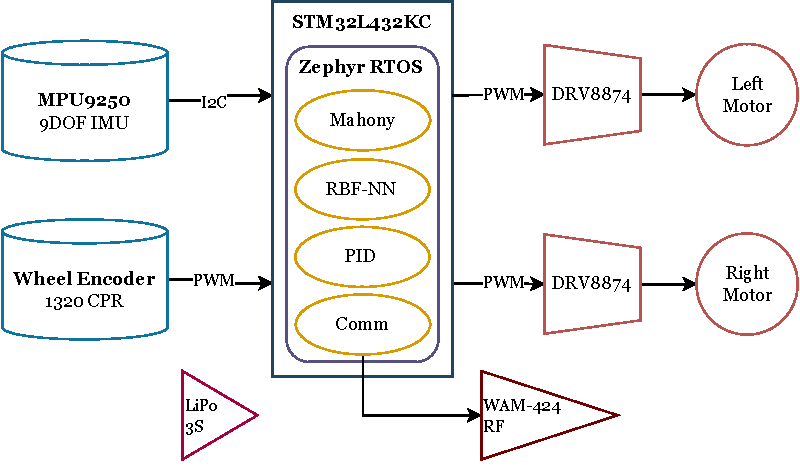
\includegraphics[width=9cm]{figures/hw_arch.pdf}
    \caption{하드웨어 아키텍처}
    \label{fig:hardware_arch}
\end{figure}
%
그림 \ref{fig:hardware_arch}은 이동식 도립 진자 하드웨어의 아키텍처입니다. 이 그림에서 휠 인코더 부분의 경우 하드웨어만 조립되고 실제 사용은 하지 않았습니다. 도립 진자의 각도 오차를 측정하기 위해 9 자유도 관성 측정 장치인 MPU9250을 사용했습니다. MPU9250는 각각 3 자유도의 가속도, 각속도, 지자계 측정 MEMS 센서를 탑재하고 있습니다. \cite{invensense:mpu9250} 여기서는 가속도, 각속도를 측정 범위(full-scale)를 각각 \(2g\), \(250rad/s\) 및 LPF를 각각 \SI{5.05}{\Hz}, \SI{5}{\Hz}로 설정해 사용했습니다. 신경망과 제어기의 연산을 처리하기 위해 마이크로컨트롤러 STM32L432KC를 사용했습니다. 이 마이크로컨트롤러는 저전력 ARM Cortex-M4 32-bit 아키텍처를 사용하며 100DMIPS 및 64KB SRAM의 준수한 성능을 가지고 있습니다. \cite{st:stm32l432kc} 액추에이터의 경우 정지 전류 약 2A 정도의 감속기 포함 모터 어셈블리인 GB37-520과 이를 제어하기 위한 40V 피크 6A 정격의 H-브릿지 모터 드라이버인 DRV8874를 사용했습니다. \cite{ti:drv8847}
%
\subsection{하드웨어 구현}
%
\begin{figure}[H]
    \centering
    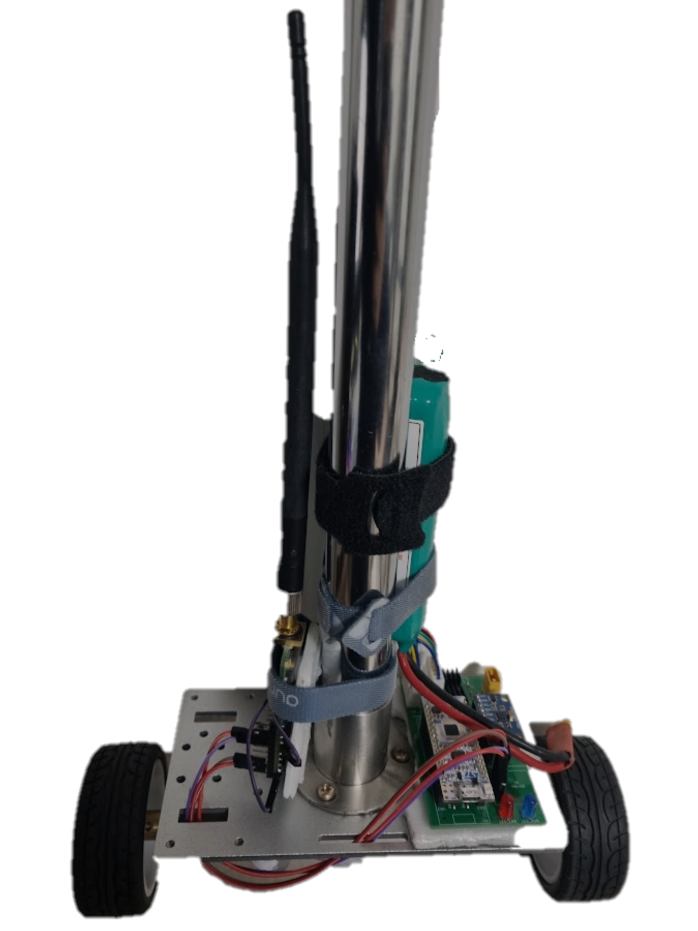
\includegraphics[width=5cm]{figures/hw.png}
    \caption{최종 하드웨어 (철봉 윗 부분이 일부 잘려있음)}
    \label{fig:hardware}
\end{figure}
%
주어진 하드웨어 아키텍처를 부록 \nameref{appendix:schematic}에 나타난 대로 회로를 설계하고 부록 \nameref{appendix:gerber}에 나타난 대로 PCB를 설계하여 제작했습니다. 알루미늄 섀시를 기반으로 진자 역할을 할 철봉을 부착하고 배터리를 장착해 그림 \ref{fig:hardware}과 같이 최종적으로 하드웨어를 제작했습니다.
%
\subsection{소프트웨어 설계}
%
\begin{figure}[h]
    \centering
    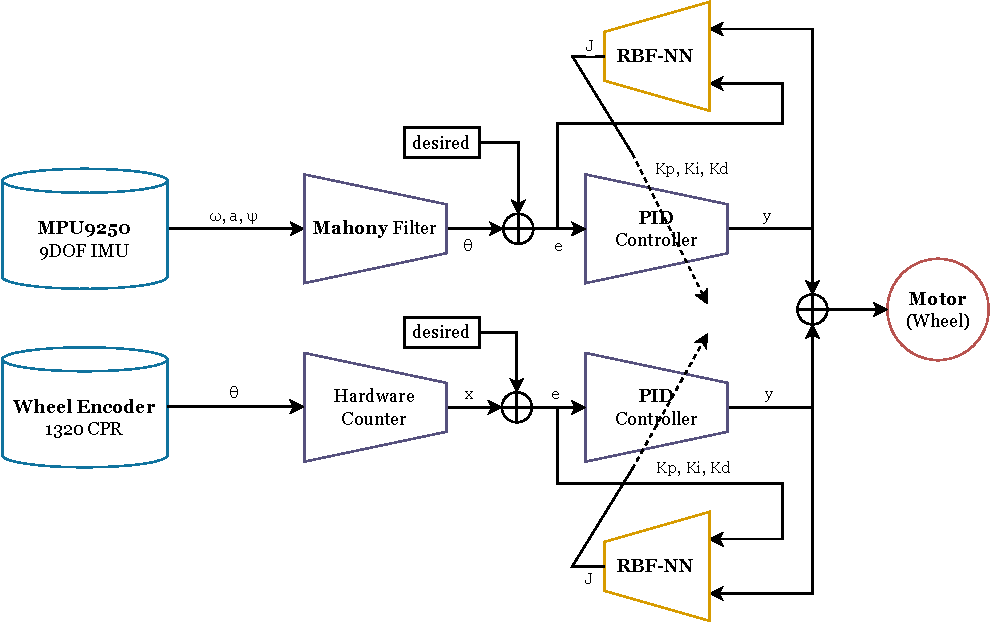
\includegraphics[width=9cm]{figures/sw_arch.pdf}
    \caption{소프트웨어 아키텍처}
    \label{fig:software_arch}
\end{figure}
%
그림 \ref{fig:software_arch}은 하드웨어에 탑재된 소프트웨어의 아키텍처를 나타냅니다. 휠 인코더 부분은 초기 설계에만 존재했고 실제 소프트웨어에서 구현되진 않았습니다. MPU9250의 여러 종류의 센서를 융합하여 자세를 산출하기 위해서 Mahony 방향 필터를 사용했습니다. 이 필터는 순간 자세와 각속도 측정에 의해 구동되는 \(SO(3)\)의 관찰자로 명시적 상보 필터를 구현하여 온라인 자이로 편향 및 자세 추정치를 제공합니다. \cite{4608934} PID 제어기와 RBF-NN의 경우 앞서 구현한 RBF 신경망을 기반으로 한 PID 제어기이며 출력값은 모터 드라이버에 지령으로 전송됩니다.
%
\begin{table}[H]
\centering
\begin{tabularx}{\linewidth}{|>{\hsize=0.5\hsize}C|
                              >{\hsize=0.4\hsize}C|
                              >{\hsize=0.7\hsize}C|
                              >{\hsize=0.4\hsize}C|} 
 \hline
 $\alpha$ & 0.25 & Mahony 필터의 $K_{p}$ & 100 \\
 \hline
 $\alpha_{g}$ & $10^4$ & Mahony 필터의 $K_{i}$ & 100 \\
 \hline
 $\eta$ & 0.05 & Mahony 필터의 $dt$ & 2ms \\
 \hline
 $K_{p}$ & 100 & 프로그램 루프의 주기 & 2ms \\ 
 \hline
 $K_{i}$ & 300 & 은닉층 노드 개수 & 8 \\ 
 \hline
 $K_{d}$ & 10 & $u_{div}$ & 500 \\
 \hline
 $B$ & 3 & & \\
 \hline
 $W$ & $10^{-2}$ & & \\
 \hline
\end{tabularx}
\caption{소프트웨어 구현에 사용된 초기 매개변수}
\label{table:sw_param}
\end{table}
%
이때 표 \ref{table:sw_param}에 나타난 \(u_{div}\)를 이용해 제어기에서 출력된 \(u\)를 식 \ref{eq_udiv}와 같이 처리하여 \(u_{motor}\)를 모터 드라이버에 지령으로 내리게 됩니다. \(u_{motor}\)은 \(u_{div}\)를 초과할 수 없습니다.
\begin{equation}
    \label{eq_udiv}
    u_{motor} = \frac{u}{u_{div}}
\end{equation}
%
\subsection{소프트웨어 구현}
%
소프트웨어는 위의 아키텍처대로 Zephyr 실시간 운영체제 위에서 동작합니다. 이 운영체제는 실시간 스케줄링 서비스 및 자료 구조, 하드웨어 드라이버와 추상화 계층 등을 제공합니다. \cite{url:zephyr} 또한 원격에서 소프트웨어의 상태 변수를 수집하기 위해 RF 무선 통신을 이용해 Golang으로 구현된 텔레메트리 소프트웨어를 구현해 사용했습니다. 구현된 소스 코드는 부록 \nameref{appendix:source}에서 수록하고 있습니다.
%
\subsection{실험}
%
\begin{figure}[H] 
    \centering
\subfloat[$K_{p}$]{
    \begin{tikzpicture}[yscale=0.7, xscale=0.7]
    \pgfplotsset{set layers}
    \begin{axis}[
        scale only axis,
        axis y line*=right,
        xlabel = 시간 (sec),
        width = 4.5cm,
        height = 5cm,
        legend style={at={(0.9, 0.4)}},
    ]
        \addplot[solid, red] table [col sep=comma, x=time, y=kp]{hardware_data.csv};
        \addlegendentry{$K_{p}$}
    \end{axis}
    \end{tikzpicture}
}
        \centering
\subfloat[$K_{i}$]{
    \begin{tikzpicture}[yscale=0.7, xscale=0.7]
    \pgfplotsset{set layers}
    \begin{axis}[
        scale only axis,
        axis y line*=right,
        xlabel = 시간 (sec),
        width = 4.5cm,
        height = 5cm,
        legend style={at={(0.9, 0.4)}},
    ]
        \addplot[solid, blue] table [col sep=comma, x=time, y=ki]{hardware_data.csv};
        \addlegendentry{$K_{i}$}
    \end{axis}
    \end{tikzpicture}
}
\subfloat[$K_{d}$]{
    \begin{tikzpicture}[yscale=0.7, xscale=0.7]
    \pgfplotsset{set layers}
    \begin{axis}[
        scale only axis,
        axis y line*=right,
        xlabel = 시간 (sec),
        width = 4.5cm,
        height = 5cm,
        legend style={at={(0.9, 0.4)}},
    ]
        \addplot[solid, black] table [col sep=comma, x=time, y=kd]{hardware_data.csv};
        \addlegendentry{$K_{d}$}
    \end{axis}
    \end{tikzpicture}
}
    \caption{실제 하드웨어에서 이득의 변화 예시}
    \label{fig:gain}
\end{figure}
%
\begin{figure}[H]
    \centering
    \begin{tikzpicture}
    \pgfplotsset{set layers}
    \begin{axis}[
        scale only axis,
        xlabel = 시간 (sec),
        ylabel = 각도 (rad) / 상대적 제어량,
        axis y line* = left,
        width = 0.8\textwidth,
        height = 4cm,
    ]
        \addplot[solid, black] table [col sep=comma, x=time, y=u]{hardware_data.csv};
        \addlegendentry{$u$}
        \addplot[solid, red] table [col sep=comma, x=time, y=e]{hardware_data.csv};
        \addlegendentry{$e$}
    \end{axis}
    \end{tikzpicture}
    \caption{시간에 따른 오차와 제어량의 변화}
    \label{fig:ue}
\end{figure}
%
구현한 실제 하드웨어와 소프트웨어를 통해 시뮬레이션과 동일한 상황을 재현함으로써 검증 실험 진행한 결과, 그림 \ref{fig:gain}과 \ref{fig:ue}와 같은 결과를 얻을 수 있었습니다. 센서의 정확도 한계와 잡음 때문에 \(\alpha_{g}\) 수치가 다르고 \(u_{div}\) 등을 도입하여 다른 경향성을 가진 결과가 도출되었으나 시스템의 출력 상황에 맞게 이득이 조절되고 올바르게 안정 상태를 유지할 수 있음을 확인했습니다.
%
%\clearpage